\documentclass[12pt]{article}

\usepackage[utf8]{inputenc}

% \usepackage[papersize={2000mm,800mm},width=2000mm,height=800mm,centering]{geometry}
% \usepackage[papersize={1000mm,400mm},width=1000mm,height=400mm,centering]{geometry}
\usepackage[papersize={500mm,200mm},width=500mm,height=200mm,centering]{geometry}

% \usepackage{mathptmx}
%\usepackage{palatino}

%\usepackage{chancery}
%\usepackage{antiqua}
%\usepackage{aboensis}
\usepackage{gfsartemisia-euler}
\usepackage[T1]{fontenc}

% \usepackage{fontspec}
% \setmainfont{QTChanceryType}

\usepackage{graphicx}
\usepackage[table]{xcolor}
\usepackage{tikz}
\usetikzlibrary{decorations.text}
\usepackage[hidelinks]{hyperref}

\pagestyle{empty}

\newcommand{\logo}{\makebox[56mm][c]{\rule{0mm}{66mm}\raisebox{12mm}{
\includegraphics[width=48mm]{logo/aldc-4couleurs-3.pdf}}}}

%\pagecolor{yellow!5}

\usepackage{fontspec}
%\usepackage{svg}

\begin{document}
%\sffamily
%\bfseries
%\color{yellow!20}
\parindent=0mm

\fontspec{QTOKCorral-Ext}
\fontsize{64pt}{64pt}
\selectfont


\unitlength=0.5mm
\begin{picture}(0,0)
%\put(-42,-450){\includegraphics[width=560mm]{desert3L.png}}
\put(-16,-444){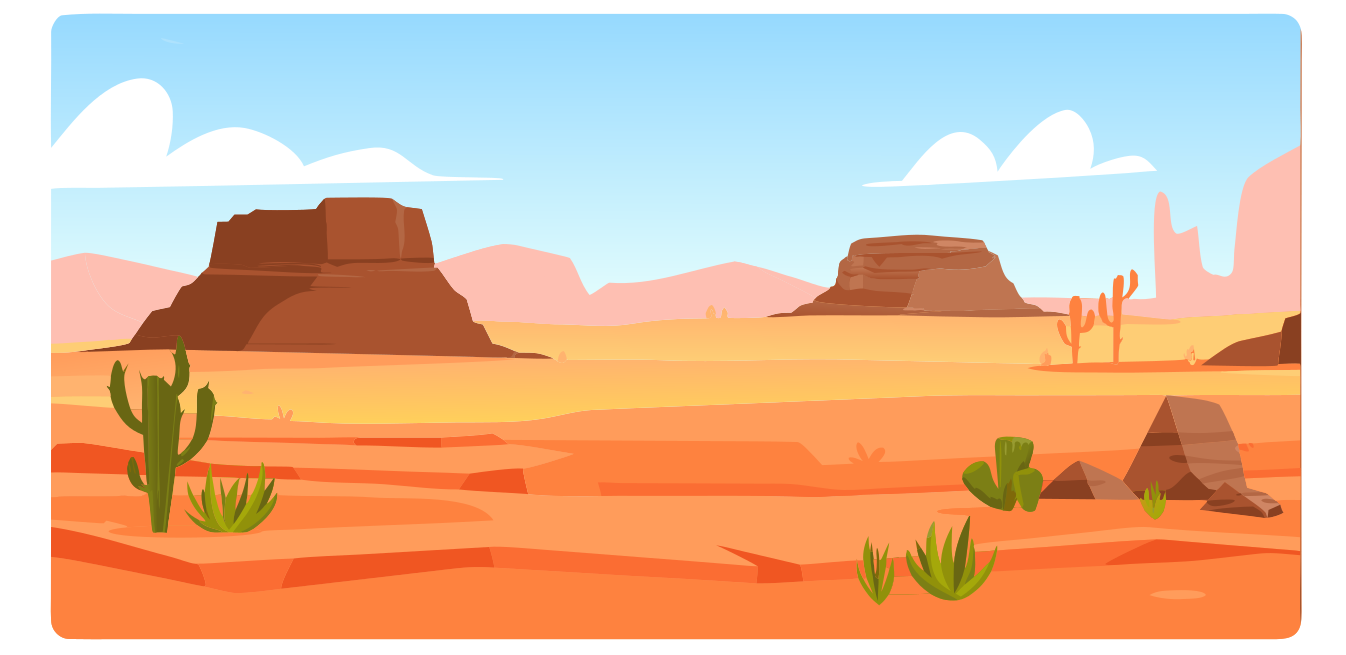
\includegraphics[width=530mm]{../images/desert3.pdf}}
%\put(10,-390){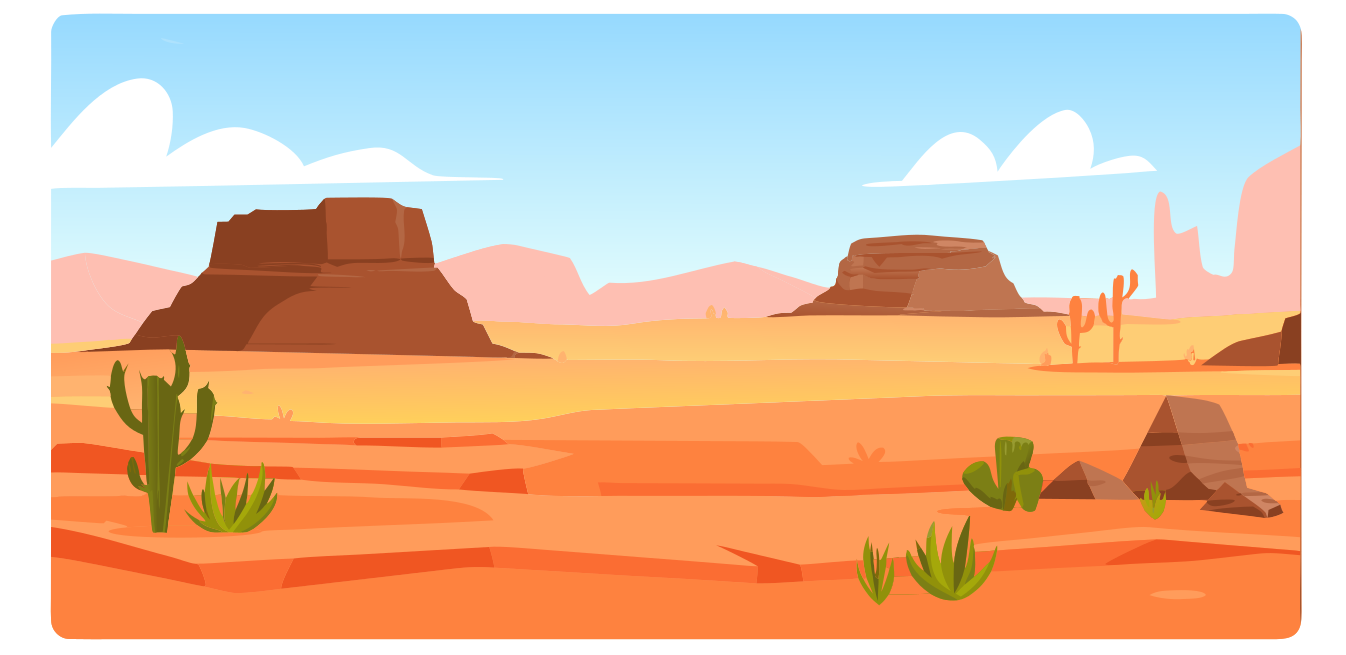
\includegraphics[height=190mm]{../images/desert3.pdf}}
\put(370,-220){\href{https://alevisdanse.github.io}{
\includegraphics[width=120mm]{../static/images/logo-aldc-contour-noir.pdf}}}
% rocher gauche
\put(180,-80){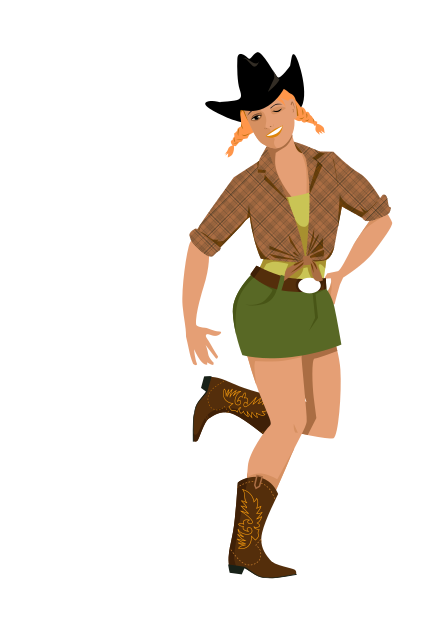
\includegraphics[height=20mm]{../images/danseur2.pdf}}
\put(250,-70){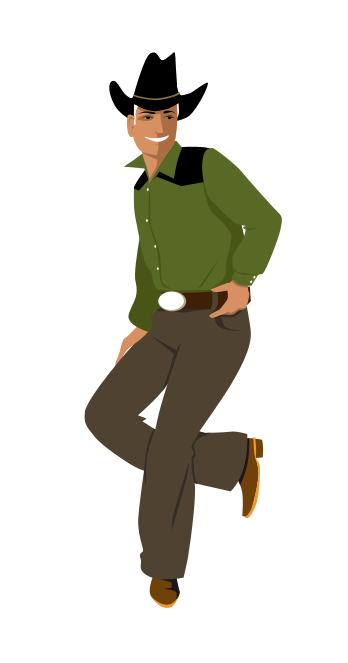
\includegraphics[height=20mm]{../images/danseur4.pdf}}
% rocher droite
\put(690,-102){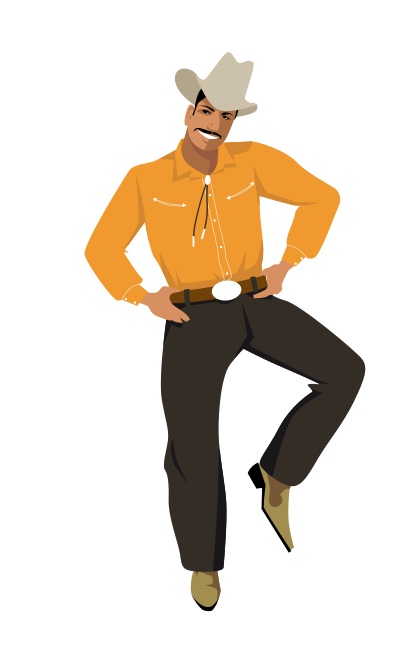
\includegraphics[height=20mm]{../images/danseur1.pdf}}
\put(745,-103){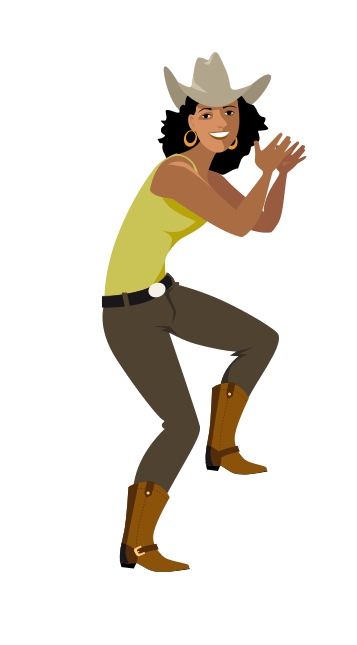
\includegraphics[height=20mm]{../images/danseur3.pdf}}
% autres
\put(210,-225){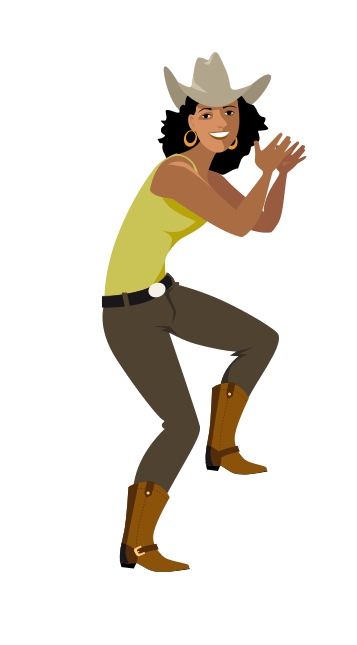
\includegraphics[height=30mm]{../images/danseur3.pdf}}
\put(310,-230){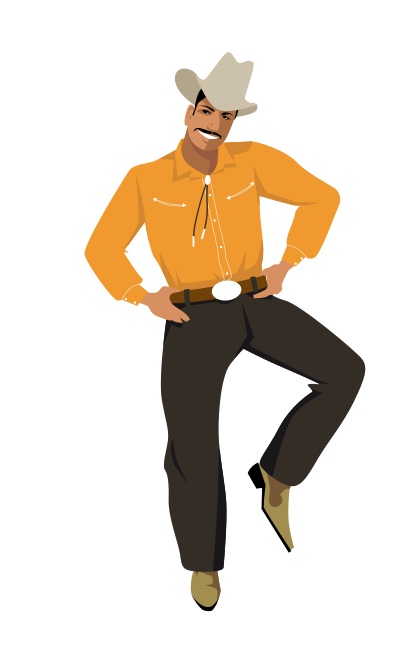
\includegraphics[height=32mm]{../images/danseur1.pdf}}
\put(655,-210){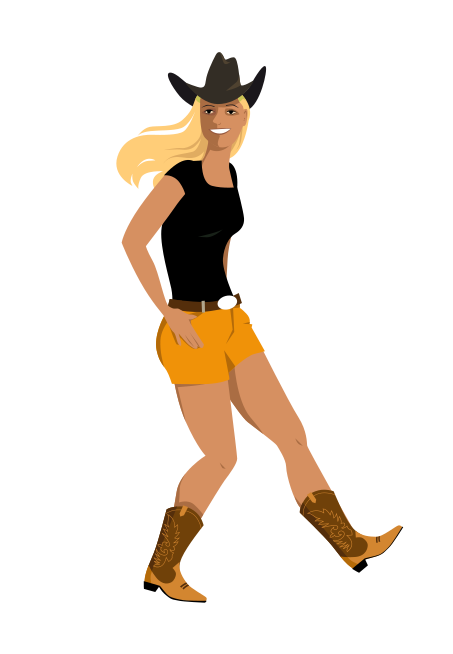
\includegraphics[height=28mm]{../images/danseur5.pdf}}
%
\put(720,-280){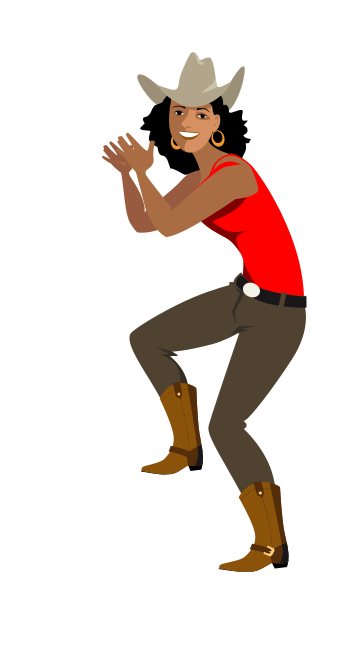
\includegraphics[height=44mm]{../images/danseur3-flip-red.pdf}}
%
\put(150,-280){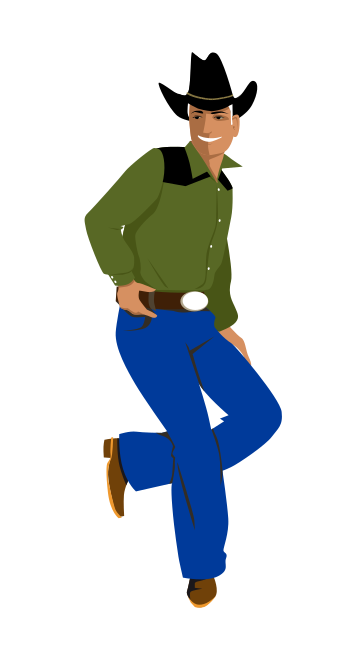
\includegraphics[height=44mm]{../images/danseur4-flip-jean.pdf}}
\put(790,-250){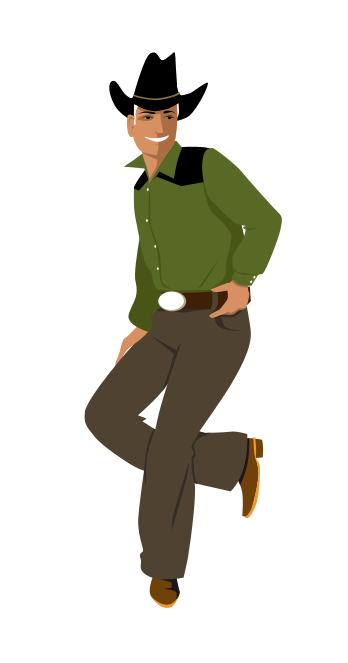
\includegraphics[height=40mm]{../images/danseur4.pdf}}
%
\put(250,-340){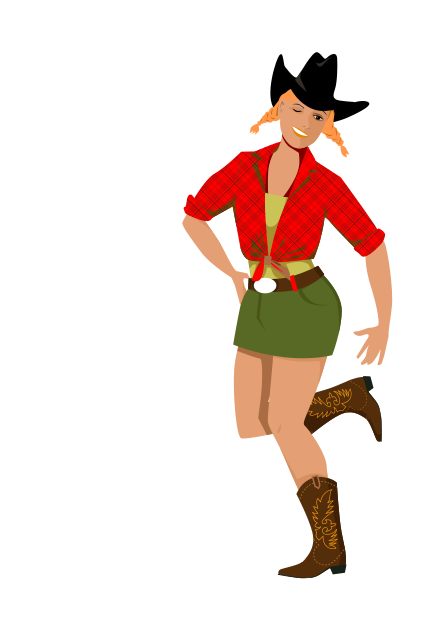
\includegraphics[height=64mm]{../images/danseur2-flip-red.pdf}}
%
\put(600,-350){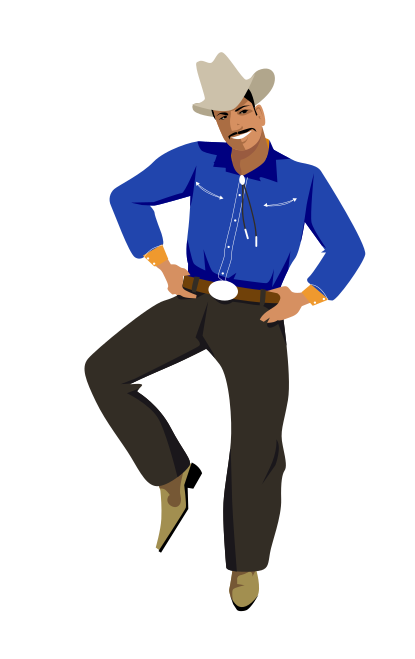
\includegraphics[height=64mm]{../images/danseur1-blue-flip.pdf}}
%
\put(370,-370){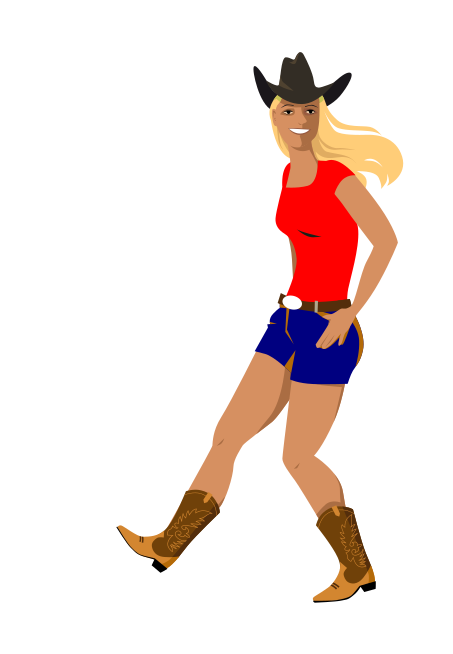
\includegraphics[height=72mm]{../images/danseur5-flip-red.pdf}}
\put(16,-380){
\includegraphics[height=16mm]{../images/qr-code.pdf}}
\end{picture}


\end{document}


%%% Local Variables:
%%% TeX-engine: luatex
%%% End: